Based on the discussions above we came up with the following final model shown
in figure~1. In this model,
figure~1 below, we aggregate the posts of 
a given user in a given thread into one document called $R_p$. 

The generative process for the figure is as follows:

\begin{figure}
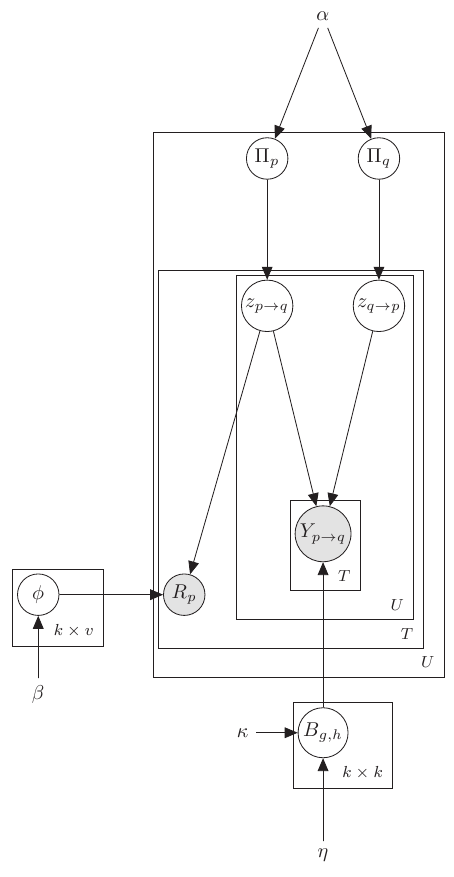
\includegraphics[0.3\textwidth]{pgm_ThreadBased.png}
\label{fig:finalThreadAggregationModel}
\caption{This graphical model takes into account multi-way interaction among
users in a thread simultaneously}
\end{figure}

Assuming that there are total $N_t$ users in the thread $t$.  
\begin{itemize}
  \item For each Thread $t$
\begin{itemize}
  \item For each user $p \in \mathcal{N}_t$
  \begin{itemize}
    \item Draw a $K$ dimensional mixed membership vector 
    $\overset{\rightarrow}{\uppi}_{p} \sim$ Dirichlet($\alpha$)

    \item Draw $B(g,h) \sim Gamma(\kappa,\eta)$; where $\kappa, \eta$ are
    parameters of the gamma distribution.
  \end{itemize}

  \item For each pair of users $(p, q) \in \mathcal{N}_t \times \mathcal{N}_t$:
  \begin{itemize}
    \item Draw membership indicator for the indicator, 
    $\overset{\rightarrow}{z}_{(p \rightarrow q,t)} \sim$
    Multinomial($\uppi_{p}$).
    \item Draw membership indicator for the receiver,
    $\overset{\rightarrow}{z}_{(q \rightarrow p,t)} \sim$
    Multinomial($\uppi_{q}$).
    \item Sample the value of their interaction, $Y(p,q,t) \sim$
    Poisson(${\overset{\rightarrow}{z}}^{\top}_{(p \rightarrow q,t)}
    B~\overset{\rightarrow}{z}_{(p \leftarrow q,t)}$). 
%     We make the assumption that
%     two interactions are independent of each other i.e $Y(p,q,i)$ and $Y(p,q,j)$
%     are independent of each other where $i\neq j$.
	\end{itemize}
	\item For each user $p \in \mathcal{N}_t$
	\begin{itemize}
	  \item Draw $\phi_{k}$ from $Dirichlet(\beta)$.
	  \item Form the set $Q_{p,t}$ that contains all the users that p interacts to
	  on thread $t$
	  \begin{itemize}
	    \item For each word $w \in R_{p,t}$ 
	    \item Draw $w \sim \phi(w|z_{(p \rightarrow q,t)}, \forall q\in Q_{p,t})$  
	  \end{itemize}
% 	  \item Draw $W \sim $
%     \item Draw $z_{u,m}$ topic for user $U$'s document from $\pi_u$.
%     \item Draw $\tau_{k}$ from $Dirichlet(\beta)$.
%     \item Draw a word $w_{u,m}$ from $\tau_{z}$
  \end{itemize}
\end{itemize}  
\end{itemize}

The data likelihood for the model in figure~1

\begin{eqnarray}
P(Y, R_{p} | \alpha, \beta, \kappa, \eta) = \int_{\Phi} \! \int_{\Pi} \sum_{z} \! P(Y, R_{p}, z_{p \rightarrow q}, z_{p \leftarrow q}, \Phi, \Pi | 
\alpha, \beta, \kappa, \eta)  \nonumber \\  \nonumber
\\ = \int_{\Phi} \! \int_{\Pi} \sum_{z} \! \bigg[ \prod_{p,q} \prod_{t}
P(Y_{pq}^{t} | z_{p \rightarrow q}^{t}, z_{p \leftarrow q}^{t}, B) 
\cdot P(z_{p \rightarrow q}^{t} | \Pi_{p}) \cdot P(z_{p \leftarrow q}^{t} |
\Pi_{q})  \nonumber
\\ \cdot \left(\prod_{p} P(\Pi_{p} | \alpha) \prod_{t} \prod_{p} P(R_{p}^{t} |
z_{p \rightarrow q}^{t}, \Phi) \cdot \prod_{k} P(\Phi_{k} | \beta)\right) \cdot
\prod_{g,h}P(B_{gh} | \eta, \kappa) \bigg]
\end{eqnarray}

The complete log likeliood of the model is:

\begin{align}
\log \! P(Y, W, z_{\rightarrow}, z_{\leftarrow}, \Phi, \Pi, B | \kappa, \eta,
\beta, \alpha) = \sum_{t} \! \sum_{p,q} \! \log P(Y_{pq}^{t} | z_{p \rightarrow
q}^{t} , z_{p \leftarrow q}^{t}, B)~+ \nonumber  \\\nonumber \sum_{t} \!
\sum_{p,q} \! (\log P(z_{p \rightarrow q}^{t} | \Pi_{p}) + \log \! P(z_{p \leftarrow q}^{t} |
\Pi_{p})) + \sum_{p} \! \log \! P(\Pi_{p} | \alpha) ~+\\  \sum_{t} \!
\sum_{p} \! \sum_{w \in R_{p}^{t}} \log P(w | z_{p \rightarrow}, \Phi) +
\sum_{k} \! \log P(\Phi_{k} | \beta) + \sum_{gh} \! \log P(B_{gh} | \eta,
\kappa)
\end{align}

The mean field variational approximation for the posterior is 

\begin{align}
q(z, \Phi, \Pi, B | \Delta_{z_{\rightarrow}}, \Delta_{\Phi}, \Delta_{B},
\Delta_{z_{\leftarrow}}, \Delta_{B_{\kappa}}) = \prod_{t} \! \prod_{p,q} \!
\bigg( q_{1}(z_{p \rightarrow q}^{t} | \Delta_{z_{p \rightarrow q}}) +
q_{1}(z_{p \leftarrow q}^{t} | \Delta_{z_{p \leftarrow q}})  \bigg) \nonumber \\
\cdot \prod_{p} \! q_{4}(\Pi_{p} | \Delta_{\Pi_{p}}) \prod_{k} q_{3} (\Phi_{k} |
\Delta_{\Phi_{k}}) \prod_{g,h} \! q(B_{g,h} | \Delta_{B_{\eta}}, \Delta_{B_{\kappa}})
\end{align}

The lower bound for the data log-likelihood from jensen's inequality is: 

\begin{align}
L_{\Delta} &= E_{q}\bigg[ \log \! P(Y, W, z_{\rightarrow}, z_{\leftarrow}, \Phi,
\Pi, B | \kappa, \eta, \beta, \alpha) - \log \! q \bigg]
\end{align}

\begin{eqnarray}
L_{\Delta} = E_{q} \left[ \sum_{t} \! \sum_{p,q} \! \log \bigg(
B_{g,h}^{Y_{p,q}^t} \frac{e^{-B_{gh}}}{Y_{pq}^{t}!} \bigg) +
\sum_{t} \! \sum_{pq} \! \log\bigg( \prod_{k} (\pi_{p,k}^{z_{p \rightarrow q} =
k}) \bigg) + \sum_{t} \! \sum_{p,q} \log \! \bigg( \prod_{k}(\pi_{q,k})^{z_{p
\leftarrow q} = k} \bigg) ~+ \nonumber\\
 \sum_{p} \! \log \left[ \prod_{k}
(\Pi_{p,k})^{\alpha_{k} - 1} \cdot \frac{\Gamma(\sum \alpha_{k})}{\prod_{k}
\Gamma(\alpha_{k})} \right] +
\sum_{t} \! \sum_{p} \! \sum_{w\in R_p^t}  \log \! \bigg(
\prod_{u\in V}(\bar{z}^T\phi_u)^{w = u} \bigg) + \nonumber\\
 \sum_{k} \! \log\left[ \prod_{u\in V}
(\phi_{k,u})^{\beta_{k} - 1} \cdot \frac{\Gamma(\sum \beta_{k})}{\prod_{k}
\Gamma(\beta_{k})} \right] +
 \sum_{g,h} \! \log \! \left( B_{g,h}^{\kappa - 1} /
\eta^{\kappa} \Gamma(\kappa) \cdot \exp(-B_{g,h}/\eta) \right) \right] 
\nonumber
\end{eqnarray}
\begin{eqnarray}
 -E_{q} \left[ \sum_{t} \! \sum_{p,q} \log \big( \prod_{k} (\Delta_{z_{p
\rightarrow q}, k})^{z_{p \rightarrow q}=k} \big) + \sum_{t} \! \sum_{p,q}
\! \log \! \big(
\prod_{k} \! (\Delta_{z_{p \leftarrow q}, k})^{z_{p \leftarrow q} = k} \big)
 + \nonumber \\
 \sum \! \log \big[ \prod_{k} \! (\Pi_{p,k})^{\Delta_{\pi_{pk}}-1}
\frac{\Gamma(\Delta_{\Pi_{p}})}{\prod_{k=1} \! \Gamma(\Delta_{\Pi_{p,k}})} \big]
 + 
\sum_{k} \log \! \big[ \prod_{u \in v}
(\Phi_{k,u})^{\Delta_{\Phi_{ku}} - 1)} \frac{\Gamma(\Delta_{\Phi_{k}})}
{\prod_{u \in v} \! \Gamma(\Delta_{\Phi_{k,u}})} \big] + \nonumber \\ 
\sum_{g,h} \log \! \big[
\frac{B_{g,h}^{\Delta_{\kappa = 1}}}{\Delta_{\eta}^{\Delta_{\kappa}}
\Gamma(\Delta_{\kappa})} \exp(-B_{g,h}/\Delta_{\eta}) \big] \right]
\label{eqn:VarLowerBound}
\end{eqnarray}

Equation~\ref{eqn:VarLowerBound} is the variational lower bound of the log
likelihood function which is to be maximized.
There are terms like $ E_q\left[\sum_{g,h} \! \log \! \left( B_{g,h}^{\kappa -
1} / \eta^{\kappa} \Gamma(\kappa) \cdot \exp(-B_{g,h}/\eta) \right) \right]$
which can be obtained by taking derivation of the partition function of the exponential
family form of gamma distribution. I still have to figure out an effective way
to evaluate $E_q\left[ \sum_{t} \! \sum_{p} \! \sum_{w\in R_p^t}  \log \! \bigg(
\prod_{u\in V}(\bar{z}^T\phi_u)^{w = u} \bigg)\right]$ which Chong suggested
(and Eric too in the last meeting) to evaluate by intriducing an additional
latent variable $\bar{z}_p$ which is a realization of the average $\frac{\sum_{q\in Q} z_{p\rightarrow q}}{|Q|}$. 
